%% Outline
% 1. Navigation is important problem
% 1.5 Traditionally addressed by mapping during exploration and path
%      planning during exploitation.
% 2. End to end learning algorithms have shown promise to take over
%      mapping and path
% 3. We do not know how these algorithms work. There has been work in computer vision that shows the learning on neural network based methods can be learning totally different kind of patterns from what we would expect.
% 4.1 We find that it is not remembering the map it is being trained on
% 4.2 We find that no path planning is  happening only, memorizing and regeneration of the sequence of steps. However, it is not 

% 1. Navigation is important problem
% 1.5 Traditionally addressed by mapping during exploration and path
%      planning during exploitation.
Navigation remains a fundamental problem in mobile robotics and artificial intelligence (\cite{SmChIJRR1986,ElCOMPUTER1980}).
The problem is classically addressed by separating the task of navigation into two steps, exploration and exploitation. 
In the exploration stage, the environment is represented as some kind of \emph{map}. 
In the exploitation stage, the map is used to \emph{plan a path} to a given destination based on some optimality criterion. 
This classical approach has been quite successful in navigation using a variety of sensors.
However, navigation in general unstructured environments, especially with texture-less \cite{YaSoKaIROS2016}, transparent and reflective surfaces \cite{lai2011large}, remains a challenge.

Recently, end-to-end navigation methods---which attempt to  
solve the navigation problem without breaking it down into separate parts of mapping and path-planning---have gained traction.
With the recent advances in Deep Reinforcement Learning (DRL), these end-to-end navigation methods, such as \cite{MnBaMiICML2016,SiHuMaNATURE2016,LePaKrISER2017,MiPaViICLR2017,OhChSiICML2016}, forego decisions about the details that are required in the intermediate step of mapping.
The potential for simpler yet more capable methods is rich; for example, the resulting trained agents can potentially optimize the amount of map information required for navigation tasks.
One such algorithm by \cite{MiPaViICLR2017} has shown promise in exploring and finding the goal efficiently within complex environments. Notably, this is done using only monocular first-person views.

\begin{figure}
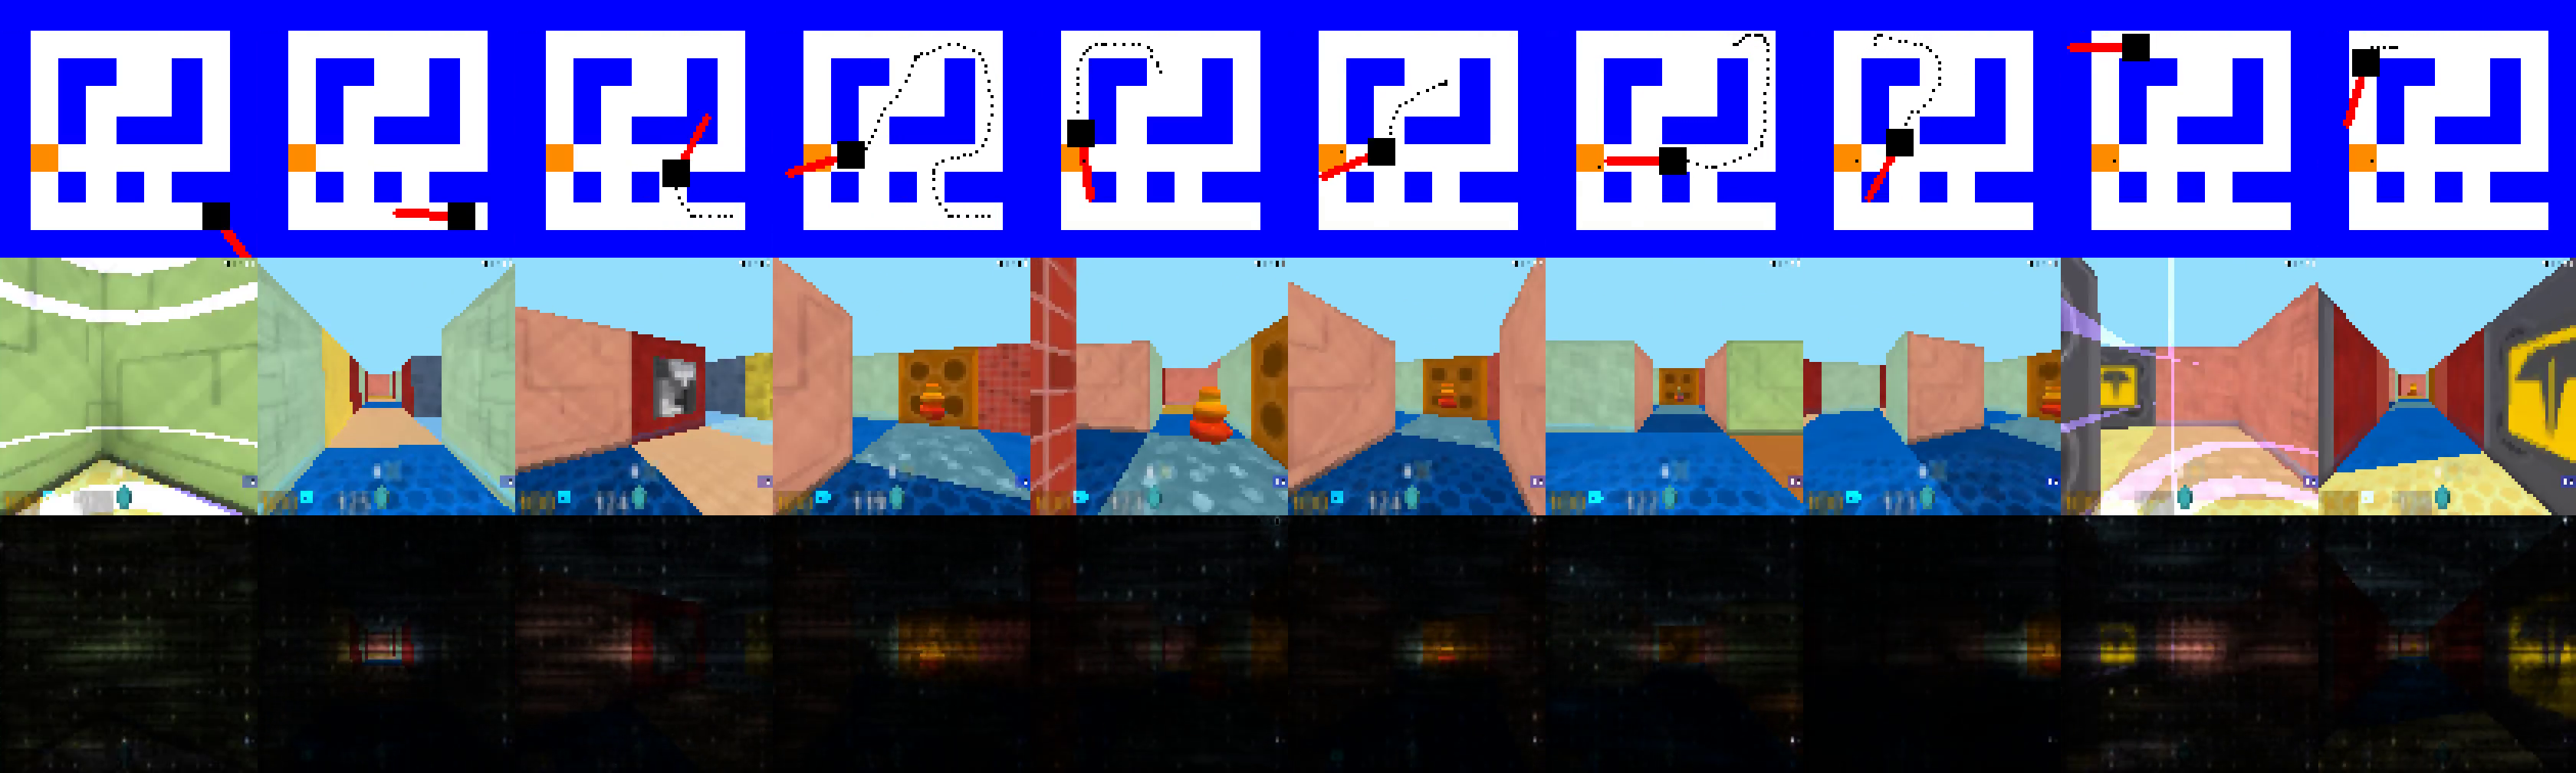
\includegraphics[width=\textwidth,trim=0 336pt 0 0,clip]{./exp-results/training-09x09-0127-on-0127.png}%
\caption{
Snapshots of the path taken by the agent while evaluating the model trained on the same random map with random goal and random spawn.
The first row shows the top view of the robot moving through the maze with the goal location marked orange, the agent marked black and the agent's orientation marked red. The second row shows the first person view, which, besides reward, is the only input available to the agent and the top view is available only for human analysis.}
\label{fig:training-qualitative}
\end{figure}

% 3. We do not know how these algorithms work. There has been work in computer vision that shows the learning on neural network based methods can be learning totally different kind of patterns from what we would expect.
Despite such potential advances, DRL-based navigation remains a relatively unexplored field with its own limitations. 
The black-box nature of these methods make them difficult to study, and the patterns captured by the methods are not well understood. 
Recent work analyzing neural networks has shown that deep learning-based object detection methods can be easily fooled by introducing noise that is imperceptible to humans (\cite{NgYoClCVPR2015}); this level of sensitivity motivates why it is particularly important to analyze DRL methods across a wide variety of experiments: we need to understand their strengths and limitations.

% 4.1 We find that it is not remembering the map it is being trained on
% 4.2 We find that no path planning is  happening only, memorizing and regeneration of the sequence of steps. However, it is not 

% Prior setup
In this work, we develop a better understanding of recent DRL-based methods. In particular, we thoroughly explore and analyze the state-of-the-art \cite{MiPaViICLR2017} methods across hundreds of maps with increasing difficulty levels. 
We set up the environment as a randomly generated map, as shown in Fig~\ref{fig:training-qualitative}, with an agent and a goal.
The agent is provided only with the first-person view and is tasked to find the goal as many times as possible within a fixed amount of time, re-spawning its location each time it reaches the goal. 
We train and evaluate the algorithms with increasing difficulty.
In the easiest stage, we keep the goal location, spawn location and map constant over the training and testing.
We call this set up \emph{static goal, static spawn, and static map}.
To increase the difficulty, we incrementally randomize the spawn locations, goal locations and map structures until all three are random.
We discuss the design of experiments in Section~\ref{sec:navtasks} in more detail.

\cite{MiPaViICLR2017} do train and test their algorithms with randomized goals and spawns and show that their algorithm is able to exploit the knowledge of the goal location at evaluation time to maximize reward.
However, following training and testing on constant map structures, this state-of-the-art result is shown to be successful on only one map, which brings into question the repeatability of the results.
It is also unclear whether these results generalize to unseen maps.

Although disjoint training and testing sets are standard practice in machine learning, to the best of our knowledge, we are the first to evaluate any DRL-based navigation method on maps with unseen structures.
We expand on the analysis in \cite{MiPaViICLR2017} to address its limitations and ask whether DRL-based algorithms such as \NavAiiiCDiDiiL{} perform any mapping followed by shortest path planning.
Our experiments show no evidence of mapping in cases where algorithms are evaluated on unseen maps and no evidence of optimal path planning, even when the map is constant and only the goal is randomized.

To better understand navigation, we compute attention-maps for models to show which portions of the input image are being used.
We find that the models discard most of the image information, focusing attention on a small band in the middle of the image except around junctions, in which case the attention is distributed evenly throughout the image.

These findings result from training and testing on multiple maps that were randomly selected from a set of 1100 randomly generated maps.
We provide experimental results on ten randomly selected maps and a testing set of 100 unseen maps to ensure results are independent of map choice.
We will make our code and data available following the blind review process.
